\documentclass[a4paper]{scrartcl}
%\documentclass[a4paper]{report}

% Uncomment to optimize for double-sided printing.
% \KOMAoptions{twoside}

% Set binding correction manually, if known.
% \KOMAoptions{BCOR=2cm}

% Localization options
\usepackage[english]{babel}
\usepackage[T1]{fontenc}
\usepackage[utf8]{inputenc}

% Enhanced verbatim sections. We're mainly interested in
% \verbatiminput though.
\usepackage{verbatim}

% PDF-compatible landscape mode.
% Makes PDF viewers show the page rotated by 90°.
\usepackage{pdflscape}

% Advanced tables
\usepackage{tabu}
\usepackage{longtable}

% Fancy tablerules
\usepackage{booktabs}

% Graphics
\usepackage{graphicx}

% Current time
\usepackage[useregional=numeric]{datetime2}

% Float barriers.
% Automatically add a FloatBarrier to each \section
\usepackage[section]{placeins}

% Custom header and footer
% \usepackage{fancyhdr}
% \setlength{\headheight}{15.2pt}
% \pagestyle{fancyplain}

\usepackage{geometry}
\usepackage{layout}

\usepackage{subcaption}

% Math tools
\usepackage{mathtools}
% Math symbols
\usepackage{amsmath,amsfonts,amssymb}

% \fancyhf{}
% % Chapter header on non-plain pages only.
% \lhead{\fancyplain{} {\leftmark}}
% % Footer must contain print date. Ugly, but IPA requirement.
% \lfoot{\printdate}
% % Print date left and page count right was the thing which looked the
% % most balanced.
% \rfoot{\thepage}
% 
% Source code & highlighting
\usepackage{listings}

% Convenience commands
\newcommand{\mailsubject}{2409 - Datenstrukturen und Algorithmen - Series 4}
\newcommand{\maillink}[1]{\href{mailto:#1?subject=\mailsubject}
                               {#1}}

% Should use this command wherever the print date is mentioned.
\newcommand{\printdate}{\today}

\subject{2409 - Datenstrukturen und Algorithmen}
\title{Series 4}

\author{Michael Senn - 16-126-880}

\date{}

% Needs to be the last command in the preamble, for one reason or
% another. 
\usepackage{hyperref}


\begin{document}
\maketitle

% \tableofcontents

\section{Illustrating Counting-Sort}

\begin{verbatim}
	A = [2, 7, 1, 3, 2, 4, 1, 8, 5, 1, 4]
	C = [3, 2, 1, 2, 1, 0, 1, 1]

	=>

	C = [3, 5, 6, 8, 9, 9, 10, 11]

	=>

	B = [, , , , , , , 4, , , ]
	C = [3, 5, 6, 7, 9, 9, 10, 11]

	=>

	B = [, , 1, , , , , 4, , , ]
	C = [2, 5, 6, 7, 9, 9, 10, 11]

	=>

	B = [, , 1, , , , , 4, 5, , ]
	C = [2, 5, 6, 7, 8, 9, 10, 11]

	=>

	B = [, , 1, , , , , 4, 5, , 8]
	C = [2, 5, 6, 7, 8, 9, 10, 10]

	=>

	B = [, , 1, , , , 4, 4, 5, , 8]
	C = [2, 5, 6, 6, 8, 9, 10, 10]

	=>

	B = [, 1, 1, , , , , 4, 5, , 8]
	C = [1, 5, 6, 7, 8, 9, 10, 10]

	=>

	B = [, 1, 1, , , , 4, 4, 5, , 8]
	C = [1, 5, 6, 6, 8, 9, 10, 10]

	=>

	B = [, 1, 1, , 2, , 4, 4, 5, , 8]
	C = [1, 4, 6, 6, 8, 9, 10, 10]

	=>

	B = [, 1, 1, , 2, 3, 4, 4, 5, , 8]
	C = [1, 4, 5, 6, 8, 9, 10, 10]

	=>

	B = [1, 1, 1, , 2, 3, 4, 4, 5, , 8]
	C = [0, 4, 5, 6, 8, 9, 10, 10]

	=>

	B = [1, 1, 1, , 2, 3, 4, 4, 5, 7, 8]
	C = [0, 4, 5, 6, 8, 9, 9, 10]

	=>

	B = [1, 1, 1, 2, 2, 3, 4, 4, 5, 7, 8]
	C = [0, 3, 5, 6, 8, 9, 9, 10]
\end{verbatim}

\section{Number of items in interval}

Let \texttt{input} = $[x_1, ..., x_n], x_i \in \{1, ..., k\}$

We start by preparing two arrays which will be used to determine the number of
items in a given interval in a later step.

\begin{verbatim}
	occurences = []
	less_than  = []

	for i = 1 to k:
	  occurences[i] = 0
	  less_than[i] = 0

	for i = 1 to n:
	  occurences[input[i]] += 1

	for i = 2 to k:
	  less_than[i] = less_than[i - 1] + occurences[i - 1]
\end{verbatim}

Clearly, the first and last loops have a time complexity of $\theta(k)$, while
the middle loop has a complexity of $\theta(n)$. As such, the preparation step
has a time complexity of $\theta(k + n)$.

Now we can calculate the number of items in the interval $[a, b]$ as:
\begin{verbatim}
	less_than[b] - less_than[a] + occurences[b]
\end{verbatim}

\section{Illustrating Radix-sort}

\begin{verbatim}
    CAT        TE*A*        M*A*P        *A*RT
    DOG        BE*D*        C*A*R        *B*ED
    CAR        DO*G*        C*A*T        *C*AR
    CUP        PI*G*        R*A*T        *C*AT
    PIG        FO*G*        D*A*Y        *C*UP
    MAP        NI*L*        T*E*A        *D*AY
    DAY        CU*P*        B*E*D        *D*OG
    ART   =>   MA*P*   =>   P*I*G   =>   *F*OG
    BED        CA*R*        N*I*L        *G*UY
    FOG        CA*T*        D*O*G        *M*AP
    GUY        AR*T*        F*O*G        *N*IL
    NIL        RA*T*        A*R*T        *P*IG
    RAT        DA*Y*        C*U*P        *R*AT
    TEA        GU*Y*        G*U*Y        *T*EA
\end{verbatim}

\section{Stability of sorting algorithms}

Implementations of insertion sort will usually be stable, since they will sort
left-to-right, moving each to-be-sorted item right-to-left until the first spot
it can fit into.
\\ 
Implementations of merge sort will usually be stable, due to - during the
merge phase - iterating over all blocks, as well as over all items within each
block - in one direction.
\\
Heapsort will not be stable, as the initial stage - where the heap is created -
will not preserve relative ordering of elements. That is, a heap provides
absolute order, but does not preserve relative one.
\\
Quicksort will not be stable, as each phase only ensures that the position of
elements relative to the pivot is correct - but makes no guarantee about the
position of elements relative to each other.

\subsection{Making unstable algorithms stable}

Comparison-based unstable sorting algorithms can be easily made stable - at the
cost of additional memory and processing time - by extending the sorting key by
the position of the item in the original input list. That is, to use the item's
original position as a 'tie-breaker' in case of items which are equal based on
their sorting key.


\section{Practical Part}

\subsection{Runtime of provided Radix sort}

The provided radix sort consists of two nested loops - the outer iterating over
each word size between 1 and the maximum word size, the inner iterating over
each item in the input.

As such, with \texttt{d} being the number of characters of the longest word,
and \texttt{c} being the number of words, we expect a total of $c * d/2 = 2*n$
iterations to take place, with \texttt{n} indicating the number of characters
total in the input. As such, complexity will be $\theta(n)$.

\subsection{Adjusted Radix sort}

The provided Radix sort was adjusted to first sort the input items by length
and then, on each iteration, to only consider those input items which are long
enough to have a character at the to-be-compared position.

This prevents having to spend time handling words whose order will not be
influenced due to lack of a character in the current column. This cuts sorting
time of bigger inputs in half.

Seen below is a test run with a small input size, showing that lexographic
sorting still works the way it did before.

\begin{verbatim}
› javac RadixSortTester.java && java RadixSortTester
  
Hopefully sorted output:
iafb
nezx
pqd
pwc
r
rt
tf
uh
w
wqgi
\end{verbatim}

\subsection{Performance of old vs new implementation}
\FloatBarrier

Both old and new implementation were timed with various inputs. These differed
in both the number of words to sort per input (plotted on the x-axis), as well
as the maximum length of each word in a given input (plotted as separate data
series each).

Clearly the new implementation is marginally slower for small data sets, due to
having to sort the input first. However, for inputs with either longer words,
or more items, it performs up to twice as fast as the original implementation.

It should be noted that, while any of the given data series seems to be growing
sligthly faster than linearly with increasing input size, the difference
between linear and actual growth is going down as input size increases. Given
that this is the case for both the old and new versions of Radix-sort, this is
likely not linked to the changes made to the algorithm.

Hence it should be safe to assume that - as intended - execution time grows
linearly with the number of characters total in the input.

\begin{figure}
    \centering
    \begin{subfigure}{.5\textwidth}
      \centering
      \caption{Runtime of old Radix-Sort}
      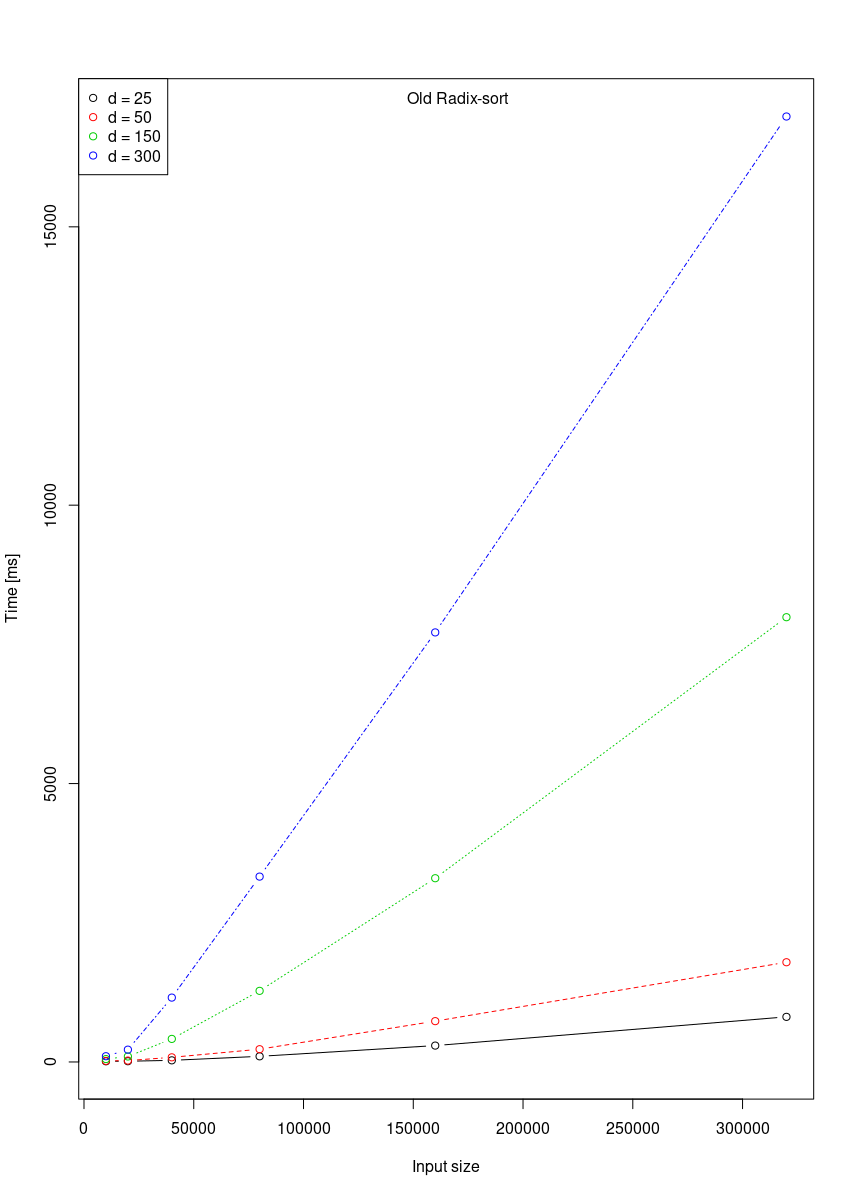
\includegraphics[width=\linewidth]{resources/runtime_old_sort.png}
    \end{subfigure}%
    \begin{subfigure}{.5\textwidth}
      \centering
      \caption{Runtime of new Radix-Sort}
      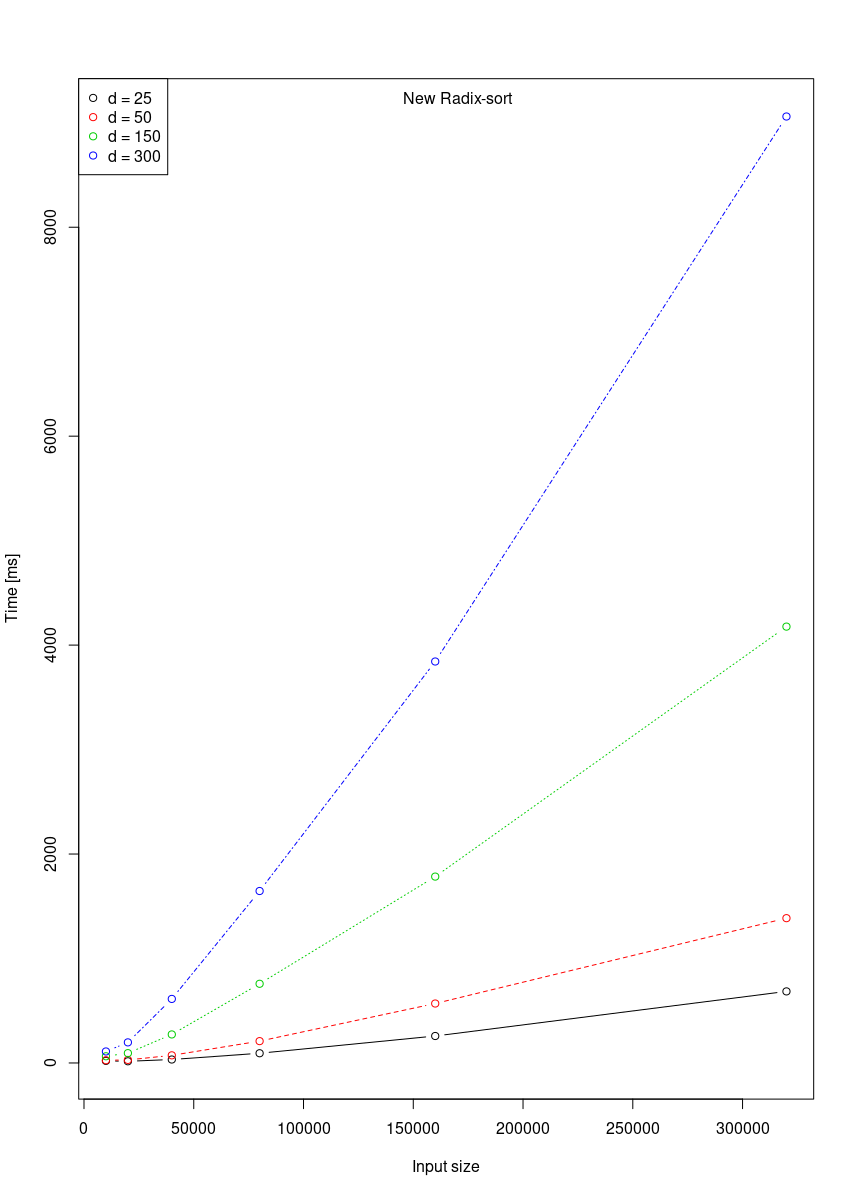
\includegraphics[width=\linewidth]{resources/runtime_new_sort.png}
    \end{subfigure}
\end{figure}

\FloatBarrier

\end{document}
